\documentclass[a4paper, 11pt]{article}

% Locale/encoding with XeTeX: UTF-8 by default, use fontspec
\usepackage{unicode-math}
\usepackage{polyglossia} % Modern replacement for Babel
\setmainlanguage{english}
\usepackage{csquotes} % guillemets
\usepackage{listings}
% Other
\usepackage{fullpage}
\usepackage{graphicx}
%\usepackage{enumerate}
%\usepackage{graphicx}
\lstset{language=Lisp}   
\begin{document}

\title{Final report on the Digital Systems course project}
\author{Nguyễn Lê Thành Dũng \and Thomas Bourgeat}

\maketitle

\section{Summary}

The project's objectives were to design a synchronous circuit usable as a general-purpose processor, and to simulate this processor at the logic gate level using a simulator we wrote ourselves. A clock program running on top of the processor would be used as a demonstration of its capabilities. Those objectives have been met.

Since there's a lot to say here, we will refer you to our two previous intermediate reports for information on the work we did previously.

What follows here is a high-level view of our architecture, combined with a rough description of how we developed the processor. All the details are confined to the appendices.

\section{What's new since last time}

\begin{itemize}
\item In the simulator, we fixed some bugs (such as memory leaks), and added all the features needed in order to run our processor at a reasonable performance (using a new execution engine using the ST Monad) and make the clock demo work.
\item In our report on the processor design, we described the kind of architecture we wanted to implement and the rough shape of its machine language. Since then, we have kept the same ideas and filled in the details, following the plans we sketched in that report to their completion.
\end{itemize}

\section{Designing an instruction set}

First, we needed to fix an instruction set that would be expressive enough for our purposes, that is, writing a clock. We concurrently developed, in a single OCaml file, a syntax tree for the S-code (our assembly language), an interpreter for this language, and a program which would count seconds and minutes. 

Our interpreter was meant as a high-level model of how our processor would work in the end. Since  we intended its source code to be amenable to mechanical translation into low-level microcode, we wrote it in an imperative style with global variables. ML-style modules were used to segregate between the memory system and the rest of the program, mirroring the Eval/GC separation in the SCHEME-79 chip \cite{SCHEME-79}.

The \texttt{ocaml/scode.ml} contains the results of this work, including, at the top, the final grammar for the S-code language. As mentioned in the previous report, a S-code program is a tree built up from words and cons cells; the \emph{tag} part of a word specifies the kind of operation to do. The tags can be classified into:
\begin{itemize}
\item Tags to annotate data with their type, e.g. numbers, lists, closures;
\item Opcodes for fundamental operations, e.g. function application, sequencing;
\item Primitive functions, e.g. consing 2 words. We included a lot of special-purpose operations for the project, such as printing a number of seconds to the clock's display.
\end{itemize}


\begin{figure}[h]
\center
\caption{Contents of a word}
   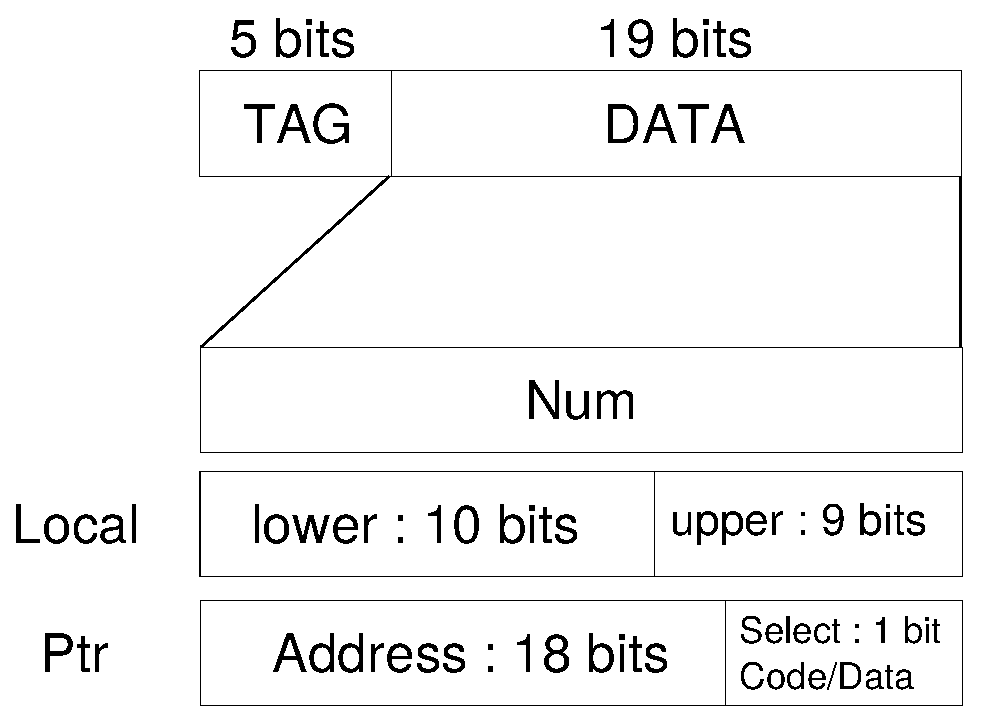
\includegraphics[scale=0.5]{words.eps}
\end{figure}


\section{From an imperative S-code interpreter to hardware}

The next step was to bridge the gap between a program running on a sophisticated runtime, and the facilities that we could provide with a circuit. On the software side, we converted non-tail function calls into explicit handling of a stack (a global variable), so as to rely only on state transitions (i.e. tail calls) for control. On the hardware side, we needed to implement:
\begin{itemize}
\item The memory system, which previously relied on OCaml's garbage collector.
\item Simple operations on numbers (incrementing and decrementing)
\item And even the mechanism to sequentially execute multiple instructions, which most programmers take for granted!
\end{itemize}
These difficulties are best illustrated by the procedure to retrieve a local variable from a pair of de Bruijn indices (a primitive in S-code): it needs to walk down a linked list, to decrement indices, and to conditionally loop!

Actually, the necessity of executing multiple elementary operations, taking a variable number of cycles, to evaluate a S-code expression led us to take inspiration from CISC processors (indeed, S-code could be considered a very complex instruction set). The technique we used was to consider the S-code instructions as initial states in a state machine encoded as \emph{microcode} and stored in a ROM. Each microinstruction consists of a number of \emph{control signals} which direct the operation of the processor in a single cycle, e.g. by controlling a multiplexer. One can see this process as compiling the relatively high-level S-code to a low-level RISC assembly on the fly.

\section{Overview of the processor}

\subsection{At the hardware level}

The processor's circuit can be divided into multiple functional units,
illustrated by figure~\ref{general}.

\begin{figure}[h]
\center
\caption{\label{general}Schematic of the general architecture.}
   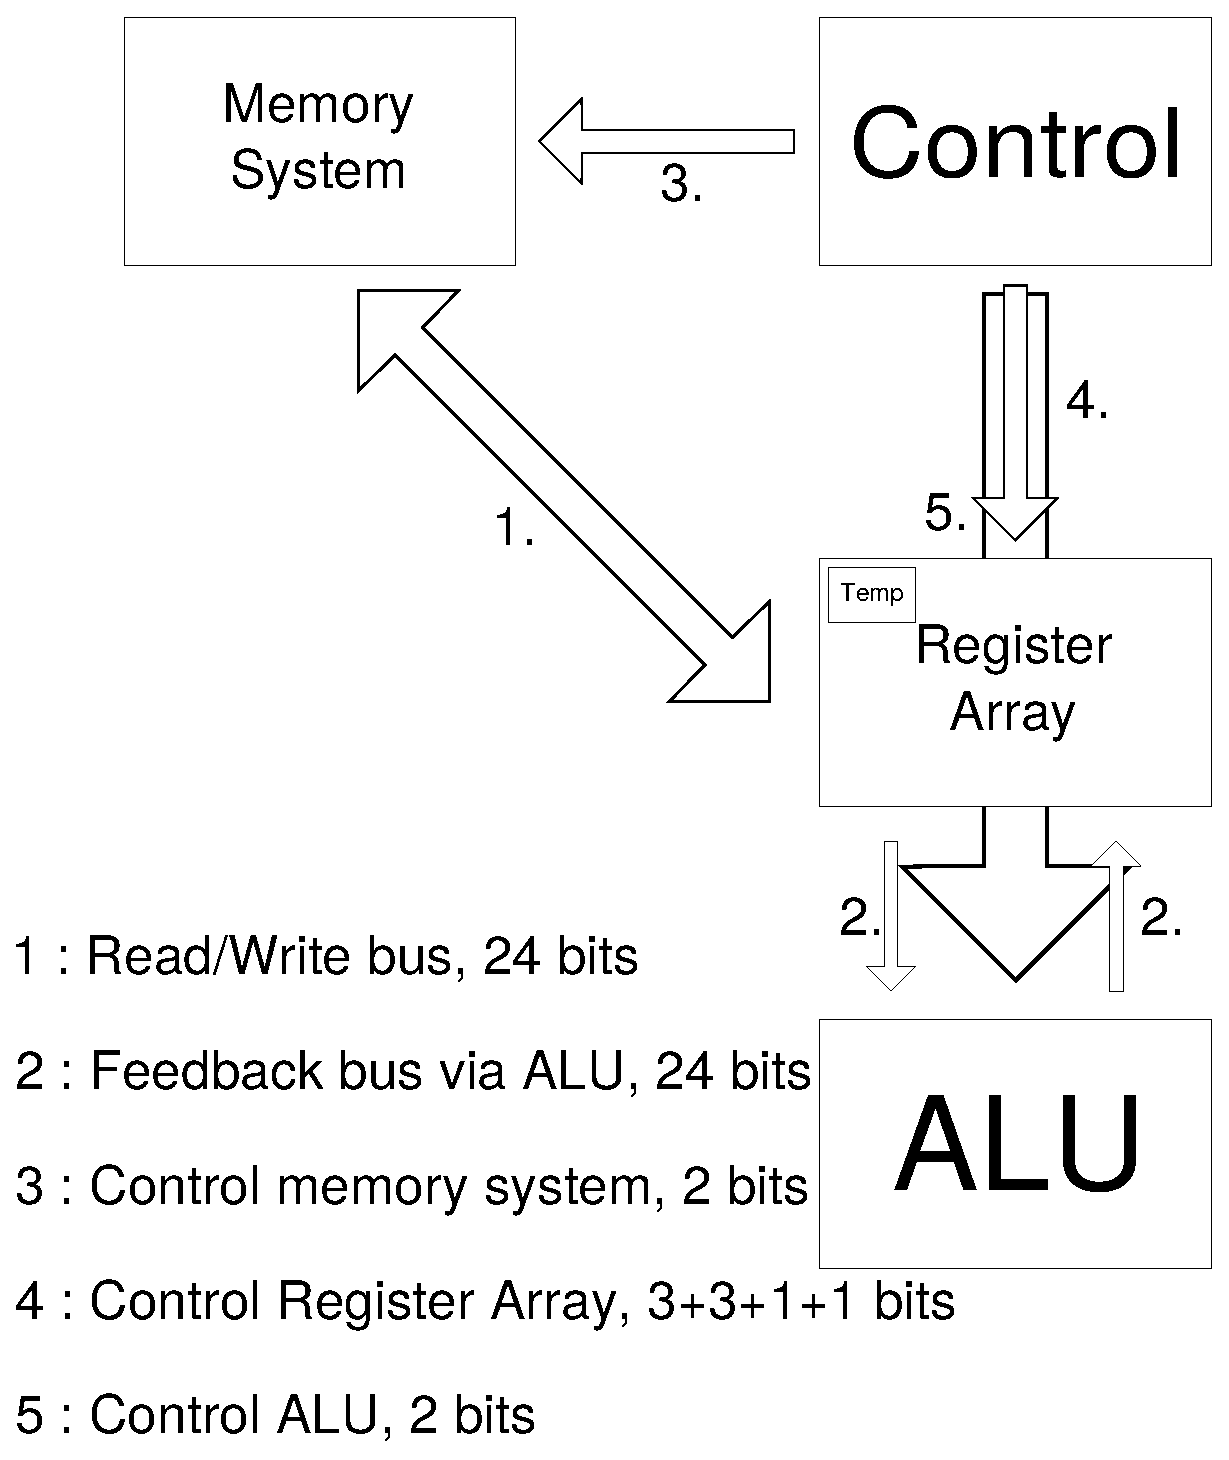
\includegraphics[scale=0.5]{globalArchi.eps}
\end{figure}

\begin{itemize}
\item The \emph{control unit}, which handles stepping through the microprogram (which is stored in a ROM), maintaining a microprogram counter. It is responsible for conditionals, and issues control signals to the rest of the processor. 
\item The \emph{memory system}, which handles anything memory-related: allocation of cons cells, and dereferencing pointers. It offers a kind of hardware-level abstraction layer: by sending the appropriate opcode, one can allocate a fresh cell without worrying finding an unused memory location. It does \emph{not} do garbage collection (even though we kept the nickname \enquote{GC} from the AI Memos), but is featureful enough to allow our clock to run indefinitely. (See appendix for details.)
\item The \emph{arithmetic logic unit} is a traditional component of any processor. Ours is very minimal, only supporting what we needed for the project. (The original SIMPLE chip \cite{SIMPLE} did not even have an ALU, nor did it need one!)
\item The \emph{register array} contains 6 registers, each containing a machine word. Although they are handled uniformly in our implementation, they are meant to be special-purpose: for example, there's a \texttt{Stack} register which holds the control stack (a pointer to a linked list), an \texttt{Expr} register which holds the current expression (analogous to a program counter)\dots There's also a special \texttt{Temp} register, used for allocating conses (for which need \emph{two} words, one from the register array and one from \texttt{Temp}).
\end{itemize}

\subsection{At the microcode level}

The microprogram is a straightforward translation of our OCaml interpreter. Pattern matching on a register's tag is simulated by cutting up the microprogram memory into segments of 32 microinstructions, each of those dedicated to reacting to a single tag, and using a dispatch mechanism to select the starting address corresponding to a tag. We also \enquote{compiled} loops into jumps, for example.

A microinstruction can either:
\begin{itemize}
\item Order around the rest of the circuit, resquesting an elementary operation from the ALU or the GC, or just moving words between registers. The control signals are retrieved from the microinstruction's binary data, without any need for decoding.
\item Jump (contionally or not). 
\item Dispatch on the tag of a register.
\end{itemize}
As can be easily seen, the processor's microcode is akin to a conventional machine language, plus a special dispatch mechanism for S-code interpretation. Indeed, we wrote the microprogram in an assembly-like language with labels (represented as Haskell lists to dispense with the need for a parser), which we then converted to binary with a (micro)assembler.


\section{The clock}

To have a clock running on the processor and displaying the current time on a graphical display, setting up some infrastructure was required both on the simulator side and on the processor side.

Relying on considerable previous experience in writing Tetris clones, we wrote a graphical program using the SDL library for the clock demo. This program, which is integrated with the simulator, shows the time given by the processor on a fake LCD display, responds to user input, and counts the time elapsed since the start of the program (so that it knows when a new second has passed). 

On the processor side, we equipped the S-code language with an instruction to wait for the next second, which allowed us to write a program counting seconds, minutes and hours in real-time. (See Appendix A for the program's source in Lisp and in S-code). This instruction triggers outputs from the processor circuit when executed. The simulator reacts to this signal by suspending the simulation, which is then resumed at the next second. 

The display program and the simulation run in two different threads, communicating using shared state.


\section{Auxiliary tools developed for the project}

In addition to the simulator, and the aforementioned graphical program, we developed some software (mostly in Haskell) to help us develop the processor and the clock:
\begin{itemize}
\item The Caillou netlist description language (already mentioned in the previous report)
\item The microassembler, to generate the contents of the microprogram ROM
\item A compiler for a very small Lisp dialect, targeting S-code (since S-code is very close to Lisp, this is a trivial syntactic transformation)
\item A S-code assembler, which linearizes the tree into binary data
\item A little program to debug the microprogram independently from the hardware
\end{itemize}


\appendix


\section{Mini-Lisp and S-Code illustrated through a minimal clock program}

Here's a little program which counts passing seconds until 60 and then stops:

\begin{lstlisting}[language=Lisp]
(defun main ()
  (count-seconds 42))

(defun count-seconds (sec)
  (print-second sec)
  (let ((new-sec (+1 sec)))
    (if (>=60? new-sec)
        ()  
        (synchronize (count-seconds new-sec)))))
\end{lstlisting}

Here is a representation of the compiled assembly. You can see the structural similarity.

\begin{figure}[h]
\center
\caption{SCode of the simplest clock}
   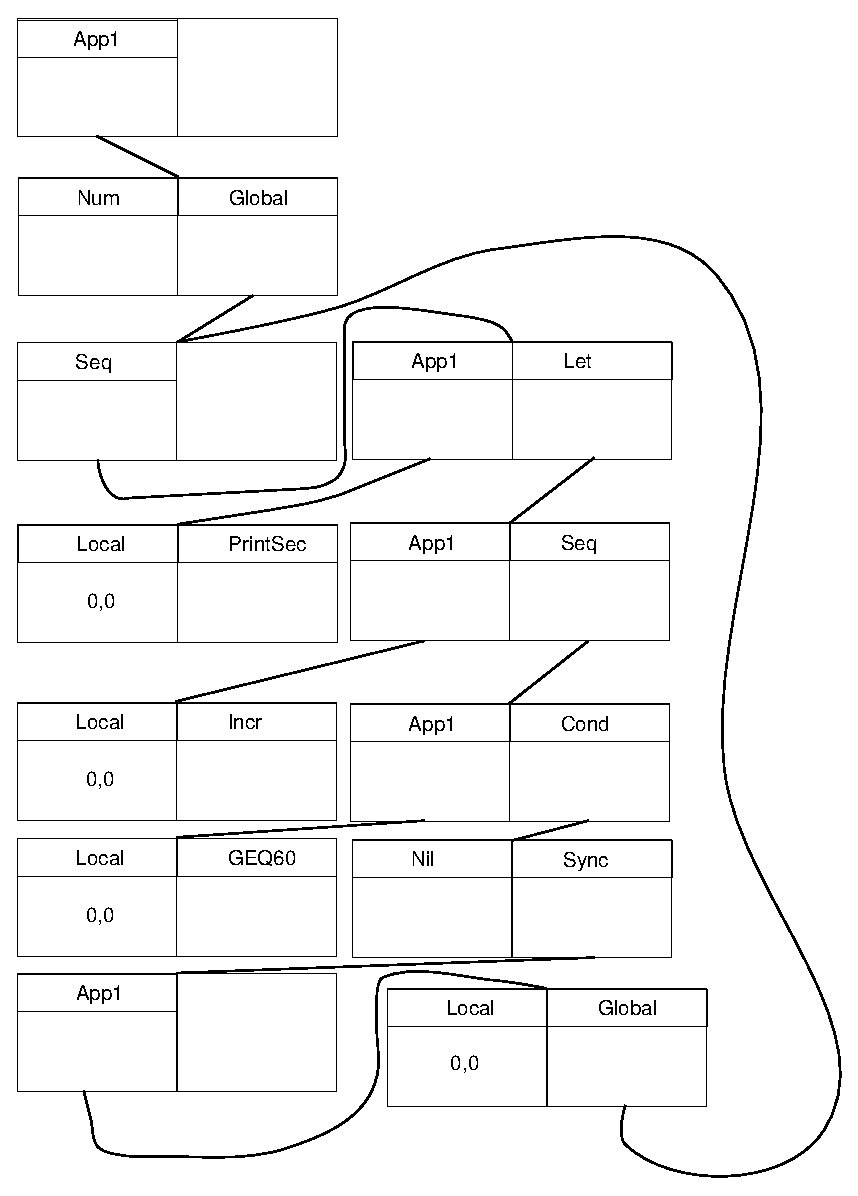
\includegraphics[scale=0.5]{clock.eps}
\end{figure}

You can see the real, more sophisticated program in "./haskell/Lisp/ClockProgram.hs".

\newpage
\section{Functional units in the processor}

\subsection{ALU}
\begin{figure}[h]
\center
\caption{Schematic of the ALU}
   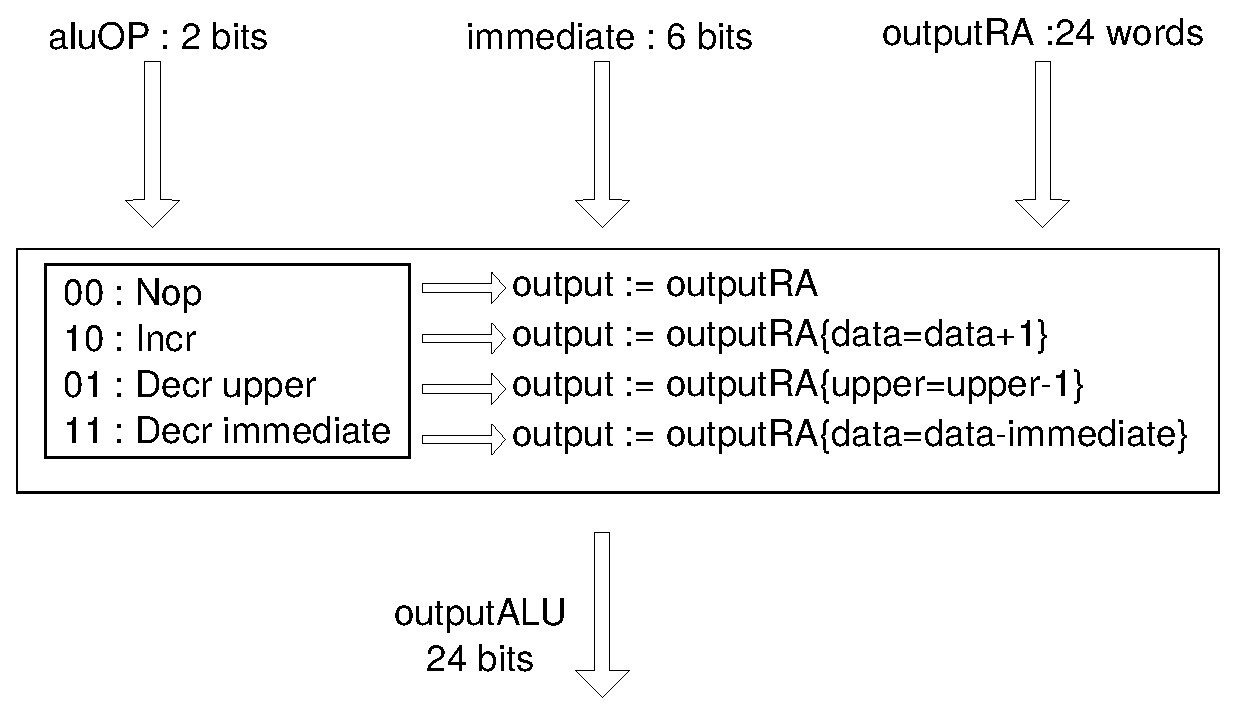
\includegraphics[scale=0.5]{ALU.eps}
\end{figure}

The ALU is very bare-bones, it can only do 4 different instructions, one of which is a special-purpose operation used only for local variables.
\begin{itemize}
\item Nop: does nothing. In this mode, the output of the ALU has the same tag as its input (so, really, it's as if it weren't there). In other modes, the output has tag Num.
\item Incr: interpreting the data part of the input (taken from the register array) as a binary number, increment it.
\item DecrUpper: decrement the 9-bit upper half of the input's data part.
\item DecrImmediate: subtract the 6-bits immediate operand from the input's data part.
\end{itemize}
Note that the Decr* operations actually output zero in case of overflow: they act like the predecessor function over the natural numbers. They also serve as comparison operations: the overflow bit, which is stored in a 1-bit register, gives the result of the comparison.

\newpage
\subsection{Memory system}

\begin{figure}[h]
\center
\caption{Schematic of the memory system}
   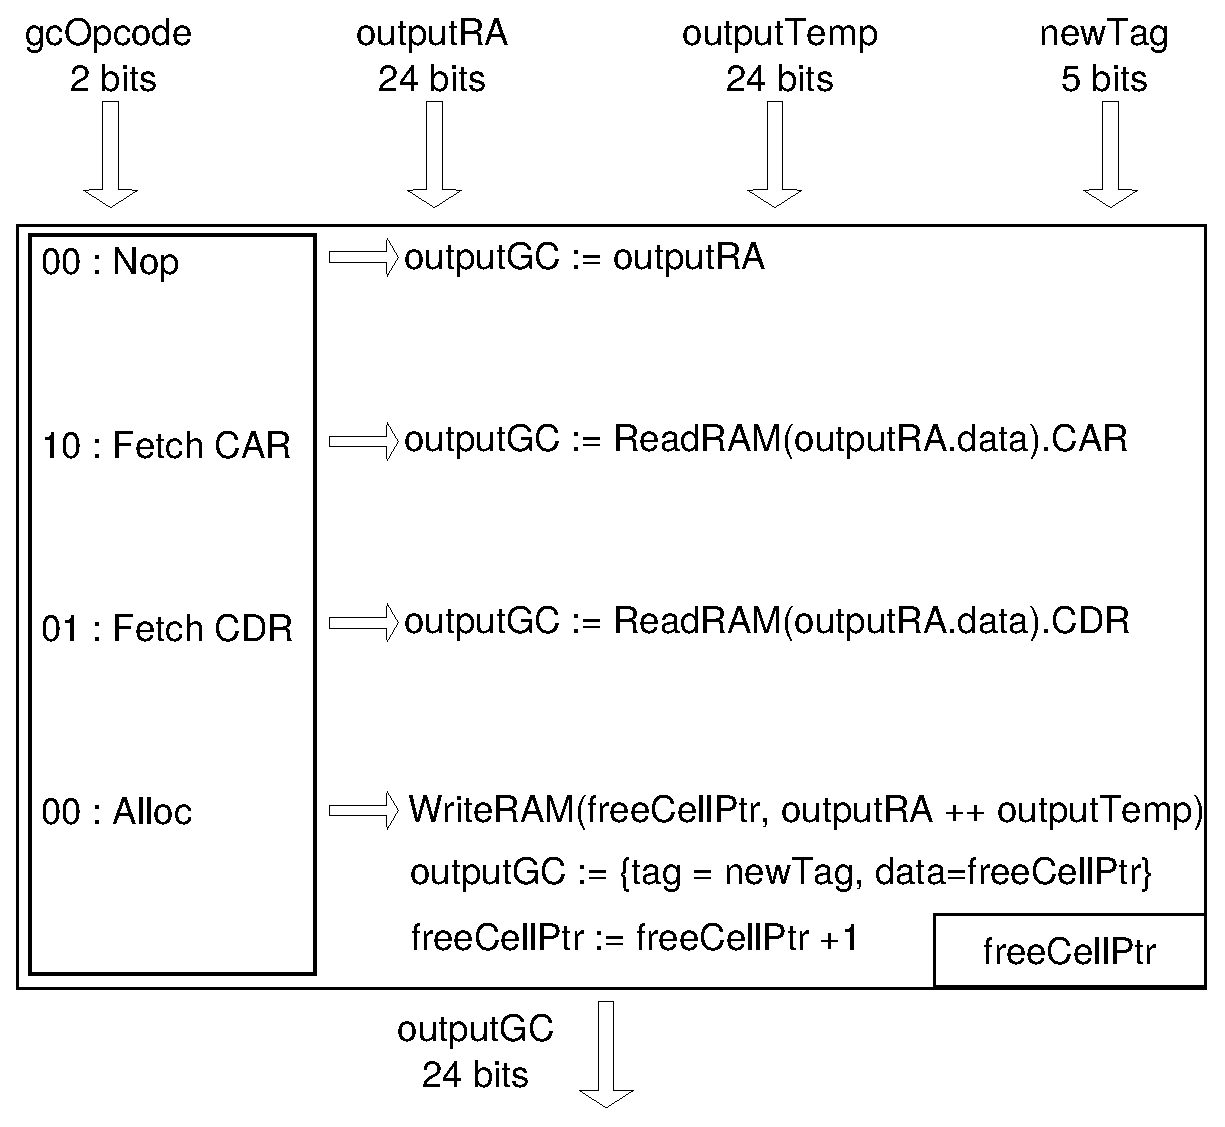
\includegraphics[scale=0.5]{GC.eps}
\end{figure}

The memory system is implemented using:
\begin{itemize}
\item A ROM array containing the S-code of the program
\item A RAM array containing the data allocated during execution
\end{itemize}
They both have a 18-bit address space; the 19th bit of a pointer selects between code and data. From the outside, it looks like a contiguous 19-bit address space with two halves.

Why do we not load both code and data into the same memory, since our machine language is homoiconic? The reasons are very pragmatic. First, we can only load ROMs with our simulator, and we need a RAM for mutable data in our memory. But it is also a hack to avoid the need for a garbage collector.

A honest memory system would provide the illusion of infinite memory by collecting unused cells with a garbage collector. What we do instead is maintain a counter to the next free cell in the RAM, which is always incremented after an allocation. When the counter exceeds the maximum address, it rewinds to zero. In general, there's no guarantee the zeroth cell isn't used, but it's true for programs which only dynamically allocate transient, short-lived data, such as our clock program. The separation of the transient data from the persistent, immutable code (which may also contain statically allocated data) makes sure this works.



\newpage
\subsection{Register Array}
\begin{figure}[h]
\center
\caption{Schematic of the register array}
   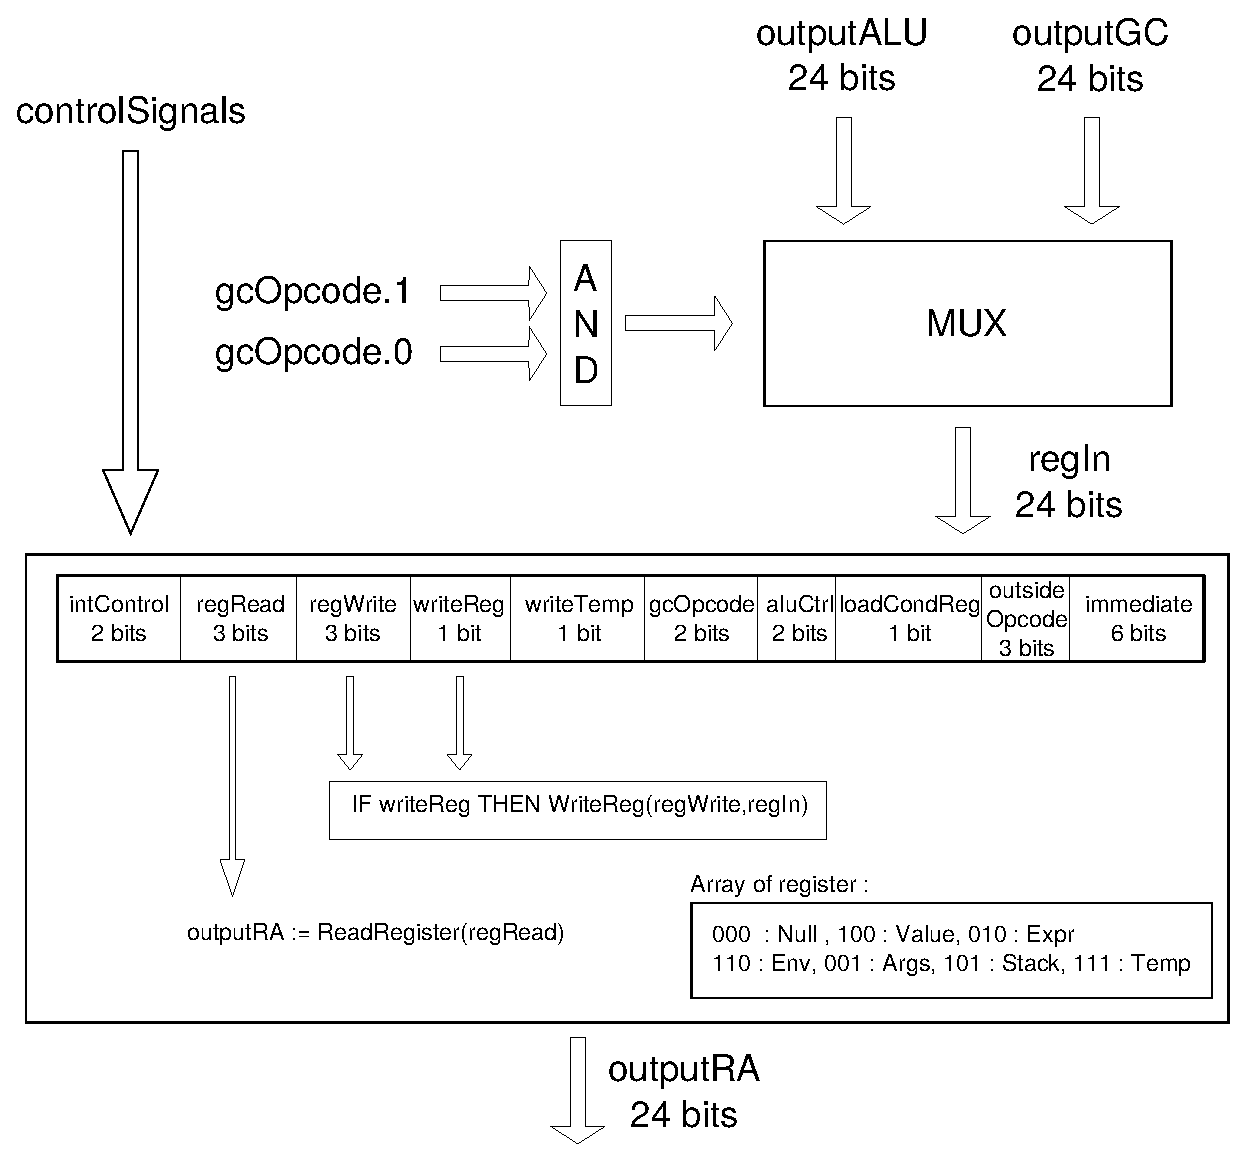
\includegraphics[scale=0.5]{RA.eps}
\end{figure}

Not much to say here. The register array is implemented in the netlist language using a RAM component with address space $2^3$, which takes care of selecting the register to read/write depending on the input on each cycle. The purposes of the registers are:
\begin{itemize}
\item Null: always contains the constant Nil
\item Value: contains the result of the last fully evaluated expression
\item Expr: the expression currently being evaluated
\item Env: the lexical environment
\item Args: list of arguments in a function call
\item Stack: the control stack
\end{itemize}


\newpage
\subsection{Control unit}
\begin{figure}[h]
\center
\caption{Schematic of the control unit}
   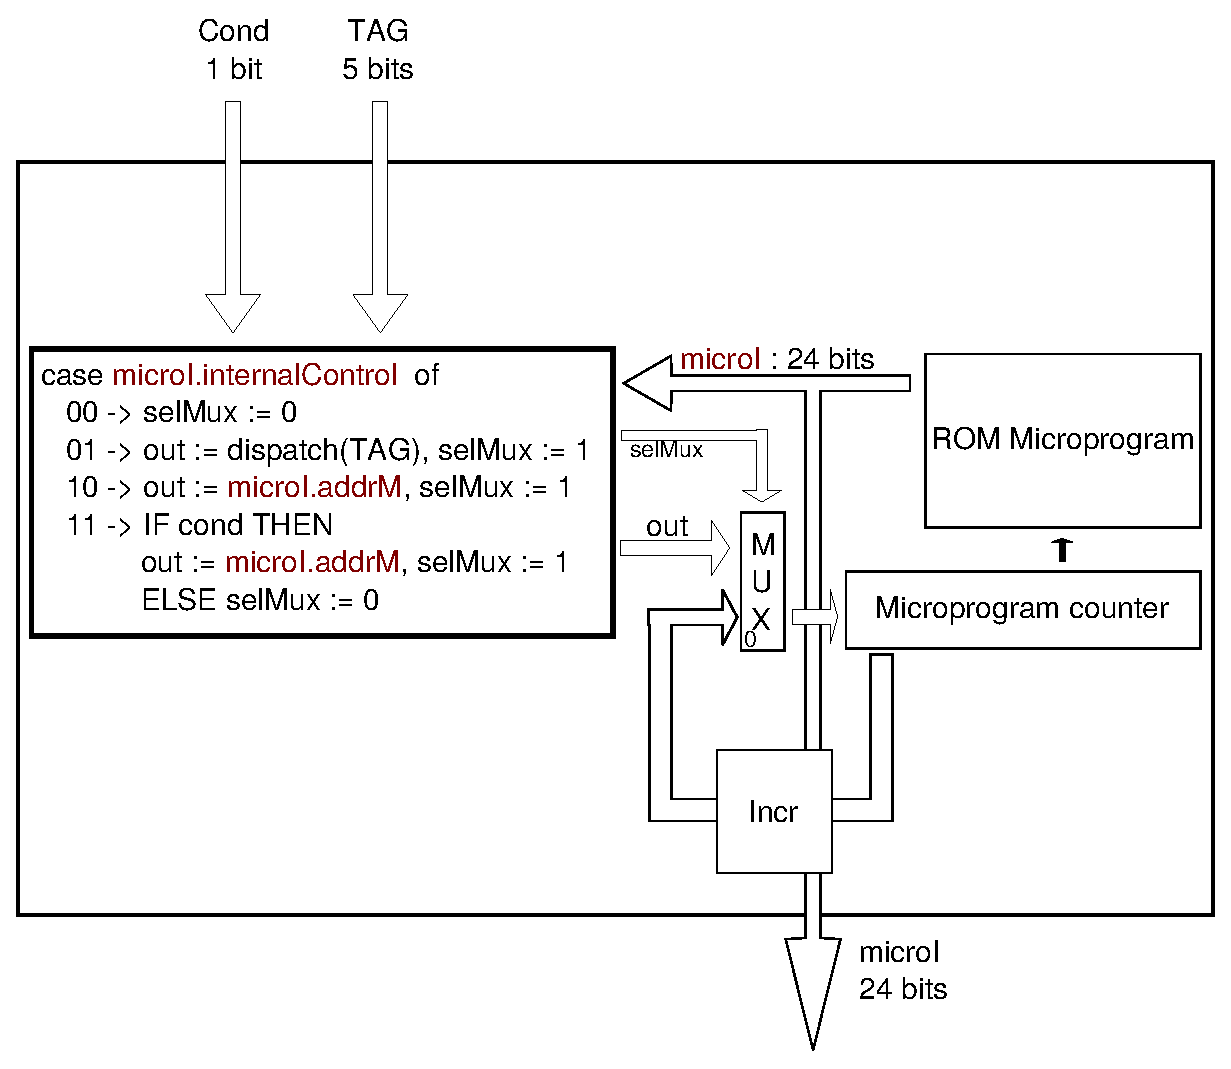
\includegraphics[scale=0.5]{control.eps}
\end{figure}


\section{Source files in the project}
\begin{itemize}
\item \enquote{README.md} : Self describing
\item \enquote{build.sh} : a script to build the entire project. It generates : rom,
simulator and processor.net. See the README for more precisions.
\end{itemize}
\subsection{./haskell}
\begin{itemize}
\item \enquote{generateRom.sh}: To generate microprogram and compile the Lisp code.
\item \enquote{simulisp.cabal}: Configuration file for cabal.
\item ./Caillou:
\begin{itemize}
\item \enquote{Arithmetic.hs}:  common arithmetical circuits
\item \enquote{Circuit.hs}: the core interface and typeclasses of Caillou
\item \enquote{Examples.hs}: some examples of elementary circuits with delays. It was a sandbox.
\item \enquote{NetlistGen.hs}: Implementation of "Circuit.hs" to generate a Netlist.
\item \enquote{Pattern.hs}: common combinators for circuits.
\item \enquote{Simulation.hs}: Implementation of "Circuit.hs" to simulate a circuit.
\end{itemize}
\item ./Lisp : 
\begin{itemize}
\item \enquote{AsmScode.hs} : Assembler number 1 from Scode to binary file.
\item \enquote{AsmScode2.hs}: Assembler number 2 from Scode to binary file. Why? Because
it's not the same algorithm!
\item \enquote{ClockProgram.hs}: The Lisp source code of the clock program. Embedded in
a haskell file using Template Haskell.
\item \enquote{MiniLispCompiler.hs}: Compiler from miniLisp to Scode.
\item \enquote{MiniLispParser.hs}: miniLisp parser
\item \enquote{MultilineQuote.hs}: Template haskell hack to include multiline string
literals such as lisp source code.
\item \enquote{Primitives.hs}: Lisp primitives
\item \enquote{SCode.hs}: the SCode grammar.  
\end{itemize}
\item ./Processor 
\begin{itemize}
\item \enquote{Hardware.hs}: Caillou description of our processor. 
\item \enquote{MicroAssembler.hs}: Assembler from microinstructions to binary file.
\item \enquote{Microde.hs}: Microprogram of our processor.
\item \enquote{Parameters.hs}: The parameters of our processor.
\item \enquote{SoftwareModel.hs}: Tool to debug the microcode independently of the
hardware implementation of the processor.  
\end{itemize}
\item ./Simulator
\begin{itemize}
\item \enquote{DisplayClock.hs}: self describing.
\item \enquote{Main.hs}: The main file: the plumbing.
\item \enquote{Scheduler.hs}: self describing.
\item \enquote{InputParser.hs}: Parser for inputs of the simulator (ROM,Inputs...)
\item \enquote{Simulator.hs}: The core of the simulator.
\item \enquote{MultiTrackDrifting.hs}: Optimized version of the simulator.
\end{itemize}
\item ./Netlist 
\begin{itemize}
\item \enquote{AST.hs}: self describing.
\item \enquote{Parser.hs}: self describing.
\item \enquote{Print.hs}: self describing.
\end{itemize}
\item ./Util
\begin{itemize}
\item \enquote{BinUtils.hs}: Tools to operate on binary numbers.
\item \enquote{Digraph.hs}: Tools to operate on directed graphs, especially topological sort.
\item \enquote{ListUtil.hs}: self describing.
\item \enquote{TopSortTest.hs}: Fun with quickcheck!
\end{itemize}
\item ./test : some old tests.
\end{itemize}

\subsection{./ocaml}
\begin{itemize}
\item \enquote{scode.ml} : Our software implementation of the processor. 
\end{itemize}
\subsection{./report}
\begin{itemize}
\item the two previous reports
\item Yours truly
\end{itemize}


\bibliographystyle{plain}
\bibliography{biblio}

\end{document}
